\documentclass[12pt,a4paper]{article}

\usepackage[a4paper, hmargin=15mm]{geometry}
\usepackage[table]{xcolor}
\usepackage{tabularx}
\usepackage{fancyhdr}
\usepackage{lastpage}
\usepackage[colorlinks=true, linkcolor=black]{hyperref}
\usepackage{tikz}

\pagestyle{fancy}
\fancyhf{}
\fancyhead[L]{\hyperref[toc]{$\leftarrow$Indice}}
\fancyhead[R]{\thepage/\pageref{LastPage}}

\rowcolors{2}{gray!10}{white}

\newcommand{\riga}[2]{
	#1 & #2\\
}

\newcommand{\tabella}[2]{
	\addcontentsline{toc}{subsection}{Comandi #1}
	\begin{center}
		\begin{tabularx}{\textwidth}{|lX|}
			\hline
			\rowcolor{gray!20}
			\textbf{#1} & \textbf{Descrizione}\\
			\hline
			#2
			\hline
		\end{tabularx}
	\end{center}
}


\title{Matematica discreta e Probabilità}
\author{Leonardo Mengozzi}
\date{}
\begin{document}
	\maketitle\thispagestyle{empty}

	\begin{center}
		\tiny Le voci dell'indice, "$\leftarrow$Indice" e i nomi delle dimostrazioni sono dei link alle rispettive sezioni.
	\end{center}

	\tableofcontents\label{toc}

	\section{Combinatoria}

\begin{quotation}
	"Serve a contare quanti elementi ci sono in un insieme.
	(risponde alla domanda "Quante sono?")."
\end{quotation}

\mysubsection{Insiemi}
Negli insiemi non conta l'ordine (infatti si usano le "\{\}", se contava l'ordine si usavano le "()") e gli elementi ripetuti. Insieme finito $\{1, \dots, n\}$. Insieme infinito $\{1,\dots\}$.

\definizione{Cardinalità}{
Un insieme $A$ ha cardinalità $n$ se contiene esattamente $n$ elementi, o equivalentemente se $\exists$ una corrispondenza biunivoca $A \longleftrightarrow \{1,2,\dots, n\}$.}{d:cardinalita}

La cardinalità si indica $|A|=n$.

\definizione{Insieme finito}{Un insieme $A$ si dice finito se $\exists n \in \mathbb{N}$ t.c. $A$ contiene esattamente $n$ elementi distinti.}{d:insiemefinito}

\osservazione{L'insieme vuoto è l'unico insieme finito di cardinalità 0.}

\definizione{Cardinalità insiemi infiniti}{
Due insiemi infiniti hanno la stessa cardinalità se $\exists$ una biezione (Corrispondenza biunivoca) tra di loro.}{d:cardinalitainsiemiinfiniti}

\definizione{Insieme numerabile}{
Un insieme $A$ si dice numerabile se ha la stessa cardinalità di $\{1,2,3,\dots\}$.}{d:insiemenumerabile}

In altre parole un insieme è numerabile se i suoi elementi possono essere messi in un a fila infinità.

Insiemi numerabili sono $\mathbb{N}$ (anche se più grande di $\{1,2,3,\dots\}$), $\mathbb{Z}=\{0,1,-1,2,-2,3,\dots\}$, $\mathbb{Q}_{>0}$ dalla dimostrazione classica di Cantor.

Un insieme non numerabile sono delle sequenze infinite di bit 0/1.

\definizione{Insieme Discreto}{Un insieme è discreto se è finito o numerabile.}{d:insiemediscreto}

\mysubsection{Combinatoria di base}
Costruisce schemi "complessi" partendo da schemi semplici riuscendo a controllarne la cardinalità. (si opera solo con insiemi finiti).

\definizione{Prodotto Cartesiano}{Siano $A, B$ insiemi il cui prodotto cartesiano $A \times B$ è l'insieme delle coppie ordinate $(a,b), a \in A, b \in B$.

generalizzando:
\[
A_1 \times A_2 \times \dots \times A_k = \{(a_1, \dots, a_k)\mid a_i\in A_i, \forall i \in 1,\dots, k\}
\]
}{d:prodcart}

\textbf{n-esima potenza cartesiana di n}, ovvero $A \times \dots \times A = A^n$.

\definizione{Sequenza}{Una sequenza (o lista) finita di lunghezza n di elementi di $A$ è un elemento $(a_1,\dots,a_n)$ del prodotto cartesiano $A^n$.}{d:sequenza}

Sono \textbf{successioni} delle sequenze di lunghezza $\infty$, tipo $\{a_1,\dots\}$.

\definizione{Insieme delle parti}{Sia $A$ un insieme, l'insieme delle parti $\mathcal{P}(A)$ è l'insieme i cui elementi sono tutti i sotto insiemi di A, inclusi l'insieme vuoto $\emptyset$ e $A$ stesso. (insieme i cui elementi sono insiemi).}{d:insiemedelleparti}

\teorema{Insieme delle parti}{Sia $A$ un insieme di $|A|=n$, allora $\exists$ una corrispondenza biunivoca tra $\mathcal{P}(A)$ e $\{0,1\}^n$.}{t:insiemedelleparti}

\dimostrazione{t:insiemedelleparti}{Vediamo un caso particolare $A=\{1,2,3\}$

$\{1\}, \{2\}, \{3\}, \{1, 2\}, \{1, 3\}, \{2,3\}, \emptyset, A$

$\updownarrow$

$100=(1,0,0),010,001,110, 101,011,000,111$

Per il caso generale $|A|=n, A=\{a_1,\dots, a_n\}$ procediamo come prima facendo corrispondere ad'un sotto insieme $S\subseteq A$ la sequenza binaria $B$ il uci i-esimo bit è $1\iff a_i\in S$.}

\mysubsection{Principi di base}
\begin{enumerate}
	\item \textbf{Principio di ugualianza:} Siano $A, B$ insiemi qualunque in corrispondenza biunivoca allora questi hanno lo stesso numero di elementi.
	\item \textbf{Principio della somma:} Siano $A, B$ insiemi qualunque disgiunti (non hanno elemtni in comune), allora $|A\cup B|=|A|+|B|$.

	Ricorda: Si dice Distinti se gli insiemi sono diversi per almeno un elemento.
	\item \textbf{Principio del prodotto:} Siano $A, B$ insiemi qualunque, allora $|A\times B|=|A|\cdot |B|$.
\end{enumerate}

Generalizzazione del Principio di ugualianza: $F:A\to B$ si dice $k:1$ (k a 1) se è surriettiva e a ogni elemento di $B$ corrispondono esattamente $k$ elementi di $A$. In questo caso $|A|=k|B|$. Il principio di ugualianza corrisponde al caso $k=1$.

\definizione{Prodotto Condizionato}{Siano $A, B$ insiemi. $C \subseteq A \times B$ è sotto insieme del prodotto cartesiano e si dice prodotto condizionato di tipo $(n,m)$ se sono soddisfatte queste condizioni:
\begin{enumerate}
	\item $\exists n$ elementi di $A$ che compaiono come 1° coefficente in un elemento di $C$.
	\item Fissata la 1° coordinata di un elemento di $C$, $\exists m$ elementi di $B$ che possono essere aggiunti come 2° coordinata.
\end{enumerate}}{d:prodcond}

In altri termini possiamo scegliere la 1° coordinata in n modi e fissata questa scelta possiamo scegliere la 2° in m modi.

Se per tutti i primi n coefficenti si hanno m secondi coefficienti si ha il prodotto condizionato, altrimenti no.

Una coordinata può non essere scelta.

\definizione{Disposizioni}{Sia $A=\{1,\dots,n\}$ una disposizione di lungheza $k$ in $A$, è una sequenza $(a_1,\dots,a_k)$ di $A$ t.c. $a_i\ne a_j, \forall i \ne j$.}{d:disposizione}

\proposizione{Fattoriale Discendente}{Le disposizioni di lunghezza $k$ in $\{1,\dots,n\}$ sono \[\underbrace{n(n-1)\cdots(n-k+1)}_{k}=(n)_k\]}{prop:fattorialediscreto}

\dimostrazione{prop:fattorialediscreto}{Abbiamo $n$ scelte per la prima coordinata. Fissata la prima coordinata ho $n-1$ scelte per la seconda coordinata. Fissate le prime due coordinate ho $n-2$ scelte per la terza coordinata, e cosi via. Abbiamo quindi un prodotto condizonato di tipo $(n,n-1,\dots,n-k+1)$.}

\definizione{Permutazioni}{Una permutazione di lunghezza $n$ è una disposizione di lunghezza $n$ in $\{1,\dots,n\}$.}{d:permutazione}

Conseguenza: Dal Fattoriale Discreto, il numero di permutazioni di lunghezza $n$ è $(n)_n=1\cdot2\dots n=n!$.

\definizione{Combinazioni}{Sia $A=\{1,\dots,n\}$, una combinazione è un sotto insieme di $A$ con $a$ elementi. (l'ordine non importa).}{d:combinazione}

\proposizione{Numero Combinazioni}{Siano $a,b,n$ con $a+b=n$, allora questi 3 insiemi sono in biezione tra loro.
\begin{enumerate}
	\item Sotto insieme di $\{1,\dots,n\}$ con $a$ elementi.
	\item Sotto insieme di $\{1,\dots,n\}$ con $n$ elementi.
	\item Sequenza binarie lunghezza $n$ con $a$ volte 1 e $b$ volte 0.
\end{enumerate}
Questi insiemi hanno esattamente $\frac{(n)_a}{a!}=\frac{(n)_b}{b!}=\frac{n!}{a!b!}$ elementi.}{prop:combinazioni}

Questo numero $\frac{(n)_a}{a!}=\binom{n}{a}=\binom{n}{a,b}$.

Coefficente binomiale:
\[
(x+y)^n=\sum_{a=0}^n\binom{n}{a}x^ay^{n-a}=\sum_{a,b\mid a+b=n}\binom{n}{a,b}x^ay^b
\]

\dimostrazione{prop:combinazioni}{$(Parte1)$ La corrispondenza tra 1 e 3 la si dimostra con il seguene esempio: $n=5, a=3$
\[
\begin{aligned}
	\{1,2,3\} \leftrightarrow 11100\\
	\{1,2,4\} \leftrightarrow 11010\\
	\{1,2,5\} \leftrightarrow 11001\\
	\{1,3,4\} \leftrightarrow 10110\\
\end{aligned}
\]
Tutte le sequenze hanno 3 "1" e 2 "0".

Poi 1 e 2 sono in biezione data dal completamento.

$(Parte2)$ Pensiamo di avere una funzione fatta cosi: Nel dominio abbiamo le disposizioni di lunghezza $a$ in $\{1,\dots,n\}$ e nel codominio abbiamo i sotto insiemi di $\{1,\dots,n\}$ con $a$ elementi. Per esempio:
\[
\begin{aligned}
	(2,5,1) \mapsto \{1,2,5\}\\
	(3,5,4) \mapsto \{3,4,5\}\\
	(3,4,5) \mapsto \{3,4,5\}\\
\end{aligned}
\]
Non è in biezione perchè non è ignettiva. (Nel caso generale abbiamo una funzione $a!:1$).

Quindi le disposizioni sono $A!$ volte i sotto insiemi e quindi i sotto insiemi con $a$ elementi sono $\frac{(n)_a}{a!}=\frac{n(n-1)\dots(b+1)}{a!}=\frac{n(n-1)\dots3\cdot2\cdot1}{a!b!}=\frac{n!}{a!b!}$.}

\definizione{Combinazione di 1\dots n}{Una combinazione di lunghezza $a$ in $\{1,\dots,n\}$ è un sotto insieme di $\{1,\dots,n\}$ con $a$ elementi.}{d:combsottoins}

\definizione{Combinazione tipo (a,b)}{Una combinazione di tipo $(a,b)$ con $(a+b=n)$ è una coppia ordinata $(A,B)$ di sotto insiemi di $\{1,\dots,n\}$ con $|A|=a,|B|=b,A\cup B=\{1,\dots,n\}$.}{d:combtipo2}

\definizione{Combinazione tipo (a,b,c)}{Una combinazione di tipo $(a,b,c)$ con $(a+b+c=n)$ è una terna ordinata $(A,B,C)$ di sotto insiemi di $\{1,\dots,n\}$ con $|A|=a,|B|=b, |C|=c,A\cup B \cup C=\{1,\dots,n\}$.}{d:combtipo3}

\definizione{Anagramma}{Sequenza ordinate di numeri $\{1,\dots,n\}$ con $n=a+b+\dots$ binarie, ternarie, quaternarie, ecc di tipo $(a,b,c,\dots)$ in biezione con le sequenze in cui compare $a$ volte "1", $b$ volte "2", $c$ volte "3", ecc.}{d:anagramma}

Esempio di riferimento (terna):
\[
\begin{aligned}
	(\{1,2\}, \{3\}, \{4\}) \leftrightarrow (1,1,2,3)\\
	(\{1,2\}, \{4\}, \{3\}) \leftrightarrow (1,1,2,3)\\
	(\{1,3\}, \{2\}, \{4\}) \leftrightarrow (1,2,1,3)\\
	(\{2,4\}, \{1\}, \{3\}) \leftrightarrow (2,1,3,1)\\
\end{aligned}
\]

\proposizione{Binomio Combinazioni tipo (a,b,c)}{Le combinazioni di tipo $(a,b,c)$ con $(a+b+c=n)$ sono $\binom{n}{a,b,c}=\frac{n!}{a!b!c!}$.}{prop:tipo3binomio}

\dimostrazione{prop:tipo3binomio}{Posso scegliere $A$ in $\binom{n}{a}$ modi. Fissato $A$ posso sciegliere $B$ in $\binom{n-a}{b}$ modi. $C$ è univocamente determinato da $A,B$.

Il numero di combinazioni di tipo $(a,b,c)$ è $\binom{n}{a}\cdot\binom{n-a}{b}=\frac{n!}{a!(n-a)!}\cdot\frac{(n-a)!}{b!(n-a-b)!}=\frac{n!}{a!b!c!}$.}

\osservazione{$\binom{n}{a,b,c}=\binom{n}{b,c,a}$=\dots, in particolare con due indici abbiamo $\binom{n}{a}=\binom{n}{b}$ se $(a+b=n)$.}

\proposizione{Somma binomi}{$\binom{n}{a,b}=\binom{n-1}{a-1,b}+\binom{n-1}{a,b-1}$ che è uguale a $\binom{n}{a}=\binom{n-1}{a-1}+\binom{n-1}{a}$.

Più in generale $\binom{n}{a,b,c}=\binom{n-1}{a-1,b,c}+\binom{n-1}{a,b-1,c}+\binom{n-1}{a,b,c-1}$.}{prop:sommabinomi}

\dimostrazione{prop:sommabinomi}{Le combinazioni di tipo $(a,b,c)$ sono in biezione con le combinazioni di tipo:
\begin{itemize}
	\item $\{(A,B,C)\mid n \in A\}$ sono $\binom{n-1}{a-1,b,c}$.
	\item $\{(A,B,C)\mid n \in B\}$ sono $\binom{n-1}{a,b-1,c}$.
	\item $\{(A,B,C)\mid n \in C\}$ sono $\binom{n-1}{a,b,c-1}$.
\end{itemize}}

\mysubsection{Cammino Reticolare}
\begin{center}
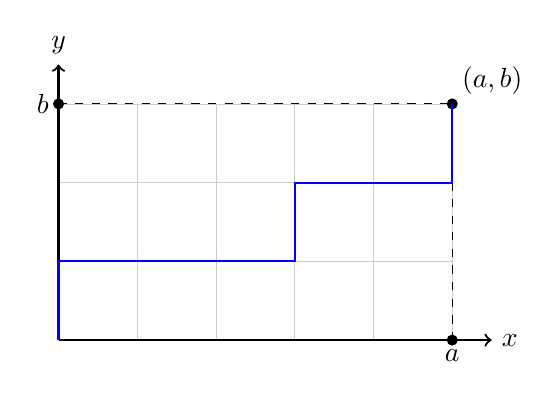
\begin{tikzpicture}[scale=1]
	% Griglia di sfondo
	\draw[step=1cm,gray!40,very thin] (0,0) grid (5,3);

	% Assi
	\draw[->,thick] (0,0) -- (5.5,0) node[right] {$x$};
	\draw[->,thick] (0,0) -- (0,3.5) node[above] {$y$};

	% Punti (0,b), (a,0), (a,b)
	\fill (0,3) circle (2pt) node[left] {$b$};
	\fill (5,0) circle (2pt) node[below] {$a$};
	\fill (5,3) circle (2pt) node[above right] {$(a,b)$};

	% Linee tratteggiate perpendicolari
	\draw[dashed] (5,0) -- (5,3);
	\draw[dashed] (0,3) -- (5,3);

	% Curva a gradini (simile a quella verde nell’immagine)
	\draw[blue,thick]
	(0,0) -- (0,1) -- (1,1) -- (2,1) -- (3,1) -- (3,2) -- (4,2) -- (5,2) -- (5,3);

\end{tikzpicture}
\end{center}

Il cammino reticolare nel piano cartesiano è il percorso che congiunge l'orgine degli assi a un punto (a,b) tramite \textit{passi} verticali o orrizontali di 1.

Ottima interpretazione grafica di una combinazione di tipo (a,b).
Quanti sono i cammini reticolari da (0,0) a (a,b)?

Possiamo codificare i passi inverticali con "1" e i passi orrizontali con "0". Cosi i cammini grafici diventano sequenze binarie. La lunghezza di tali sequenze è $a+b$, con $a$ volte "0" e $b$ volte "1". Abbiamo ottenuto un anagramma di tipo (a,b).

Osserviamo che abbiamo una biezione tra cammini e anagrammi e i cammini sono quindi $\binom{a+b}{a,b}$.

\mysubsection{Numeri di Fibonacci}
Conta i sotto insiemi di $\{1,\dots,n\}$ che non hanno 2 numeri consecutivi.

\[F_n=\sum_{k=0}^n\binom{n-k+1}{k}\]

\textbf{Ragionamento}, Definiamo:

\begin{itemize}
	\item $F_n$ come il numero di sotto insiemi possibili di $\{1,\dots,n\}$.
	\item $F_{n,k}$ il numero di sotto insiemi di $\{1,\dots,n\}$ di $k$ elementi che non hanno due elementi consecutivi.
\end{itemize}

Arriviamo alla formula con un esempio, $F_{8,3}$. Vediamo questi insiemi come sequenze di lunghezza 8 con 3 "1" non consecutivi (astrazione simile Camminio Reticolare). Devo riuscire ad'usare il principio d'equivalenza con un insieme di cui so la cardinalità. Sò che dopo il primo e secondo "1" c'è sempre uno "0", quindi cancello questo "0" cosi ho sequenze da 6.
Ora "1" possono essere consecutivi ma posso tornare univocamente alla precedente rappresentazione, quindi è biunivoco.
Deduciamo che $F_{8,3}=\binom{6}{3}=20$.

In generale $F_{n,k}$ sono le sequenze di lunghezza $n$ con $k$ volte "1", non consecutivi. Cancellando gli "0" che seguono i primi $k-1$ "1" otteniamo una sequenza binaria lunga $n-k+1$, con $k$ "1".

Tali sequenze sono $F_{n,k}=\binom{n-k+1}{k}$ e quindi $F_n=\sum_{k=0}^n\binom{n-k+1}{k}$.
A $n$ non ci arrivo perchè il coefficente binomiale da 0 quando $k>n-k+1$.
	\section{Statistica Descrittiva}

\begin{quotation}
	"Si occupa di presentare/descrivere i dati raccoli in un indiagine nel modo migliore possibile (sintetico, comunicativo)."
\end{quotation}

\definizione{Popolazione}{Insieme su cui vogliamo effettuare un'indagine.}{d:popolazione}

\definizione{Carattere}{Un carattere è quello che vogliamo studiare dalla popolazione.}{d:carattere}

\begin{itemize}
	\item \textbf{Carattere Quantitativo} se assumiamo valori numerici che esprimono una misura.
	\item \textbf{Carattere Qualitativo} se non è qualitativo.
\end{itemize}

I caratteri sarebbero distinguibili anche in \textbf{discreti e continui}.

\definizione{Unità (Statistica)}{Un unità (statistica) è un elemento della popolazione.}{d:uniStatistica}

\definizione{Campione}{Un campione è un sotto insieme (rappresentativo) della popolazione del quale possiamo determinare il valore del campione.}{d:campione}

\definizione{Modalità}{La modalità sono i valori che può assumere il carattere.}{d:modalità}

\definizione{Classi}{Se le modalità sono molto numerose (o infinite) è conveniente raggrupparle in \textbf{classi}.

Una classe, solitamente, è determinata dal \textbf{confine inferiore e superiore}.
Il \textbf{valore centrale} di una classe è la media dei confini.

Se abbiamo un solo confine chi fa l'indagine può decidere un valore rappresentativo come valore centrale.}{d:classi}

\definizione{Frequenza (assoluta)}{La frequenza (assoluta) di una modalità è il numero di volte in cui compare nel campione.}{d.freqAss}

\definizione{Frequenza relativa}{La frequenza relativa è il rapporto fra la frequenza assoluta e la cardinalità del campione. \[F_R=\frac{F_A}{|campione|}\]}{d:freqRel}

\definizione{Istogramma}{L'istogramma è un grafico che rappresenta i risultati di un'indagine.

Ad'ogni modalità (classe) è associato un rettangolo con base proporzionale all'ampiezza e area proporzionale alla frequenza.}{d:istogramma}

\begin{center}
	\begin{tikzpicture}
		\draw[draw=black, -latex, thin, solid] (-5.00,0.00) -- (5.00,0.00);
		\node[black, anchor=south west] at (-5.06,-0.75) {0};
		\node[black, anchor=south west] at (-4.06,-0.75) {10};
		\node[black, anchor=south west] at (-3.06,-0.75) {20};
		\node[black, anchor=south west] at (-2.06,-0.75) {30};
		\node[black, anchor=south west] at (-1.06,-0.75) {40};
		\node[black, anchor=south west] at (-0.06,-0.75) {50};
		\node[black, anchor=south west] at (0.94,-0.75) {60};
		\node[black, anchor=south west] at (1.94,-0.75) {70};
		\node[black, anchor=south west] at (2.94,-0.75) {80};
		\node[black, anchor=south west] at (3.94,-0.75) {90};
		\draw[draw=black, thin, solid] (-5.00,0.00) circle (0.1);
		\draw[draw=black, thin, solid] (-4.00,0.00) circle (0.1);
		\draw[draw=black, thin, solid] (-3.00,0.00) circle (0.1);
		\draw[draw=black, thin, solid] (-2.00,0.00) circle (0.1);
		\draw[draw=black, thin, solid] (-1.00,0.00) circle (0.1);
		\draw[draw=black, thin, solid] (0.00,0.00) circle (0.1);
		\draw[draw=black, thin, solid] (1.00,0.00) circle (0.1);
		\draw[draw=black, thin, solid] (2.00,0.00) circle (0.1);
		\draw[draw=black, thin, solid] (3.00,0.00) circle (0.1);
		\draw[draw=black, thin, solid] (4.00,0.00) circle (0.1);
		\draw[draw=black, thin, solid] (-5.00,0.00) -- (-5.00,2.00);
		\draw[draw=black, thin, solid] (-5.00,2.00) -- (-3.00,2.00);
		\draw[draw=black, thin, solid] (-3.00,2.00) -- (-3.00,0.00);
		\draw[draw=black, thin, solid] (-3.00,1.50) -- (-1.00,1.50);
		\draw[draw=black, thin, solid] (-1.00,1.50) -- (-1.00,0.00);
		\draw[draw=black, thin, solid] (-1.00,0.50) -- (1.00,0.50);
		\draw[draw=black, thin, solid] (1.00,0.50) -- (1.00,0.00);
		\draw[draw=black, thin, solid] (1.00,0.50) -- (1.00,3.00);
		\draw[draw=black, thin, solid] (1.00,3.00) -- (2.00,3.00);
		\draw[draw=black, thin, solid] (2.00,3.00) -- (2.00,0.00);
		\draw[draw=black, thin, solid] (2.00,3.00) -- (2.00,3.50);
		\draw[draw=black, thin, solid] (2.00,3.50) -- (2.50,3.50);
		\draw[draw=black, thin, solid] (2.50,3.50) -- (2.50,0.00);
		\draw[draw=black, thin, solid] (2.50,1.50) -- (4.00,1.50);
		\draw[draw=black, thin, solid] (4.00,1.50) -- (4.00,0.00);
	\end{tikzpicture}
\end{center}

\definizione{Media Campionaria}{La media campionaria si effettua su un carattere quantitativo su un campione di $n$ elementi. \[\overline{x}=\overline{x}_n=\frac{1}{n}(x_1+\dots+x_n)\]}{d:medCamp}

Ricordiamo delle proprietà delle sommatorie:
\begin{itemize}
	\item $\sum_{i=1}^n(a_i+b_i)=\sum_{i=1}^na_i+\sum_{i=1}^nb_i$
	\item $\sum_{i=1}^nc=nc$
	\item $\sum_{i=1}^n(ca_i)=c\sum_{i=1}^na_i$
	\item $\sum_{i=1}^n(\sum_{j=1}^n(a_ib_j))=(\sum_{i=1}^na_i)\cdot(\sum_{i=1}^nb_i)$
\end{itemize}

\definizione{Linearità della media}{Siano $x,y,z$ tre caratteri legati dalla relazione $z=ax+by$ con costanti $a,b$. \[\overline{z}=a\overline{x}+b\overline{y}\]}{d:linMed}

Caso particolare è con $y=1$ ottenendo così $z=ax+b$ e quindi $\overline{z}=a\overline{x}+b$. Può essere usato per semplificare i conti.

\dimostrazione{d:linMed}{\[\overline{z}=\frac{1}{n}\sum_{i=1}^nz_i=\frac{1}{n}\sum_{i=1}^n(ax_i+by_i)=\frac{1}{n}a\sum_{i=1}^nx_i+\frac{1}{n}b\sum_{i=1}^ny_i=a\overline{x}+b\overline{y}\]}

\definizione{Media Ponderata}{La media ponderata si usa per dare diversa importanza (peso) ai vari elementi d'un campione. \[\overline{x_w}=\frac{x_1w_1+\dots+x_nw_n}{w_1+\dots+w_n}\]}{d:medPond}

\osservazione{La media campionaria si ottiene dando peso 1 a tutti gli elementi.}

\definizione{Varianza}{La varianza di $x$ è la media dei quadrati della distanza da $\overline{x}$. \[\sigma_x^2=\frac{1}{n}\sum_{i=1}^n(x_i-\overline{x})^2\]}{d:varianza}
In altre parole indica la dispersione dei valori, ovvero da una misura di qunato i dati sono lontanti tra dolo.

\dimostrazione{d:varianza}{Ricordiamo la formula della parabola $at^2+bt+c=0, a>0$ e con vertice d'ascissa $-b/2a$.

Possiamo fissare un punto a caso $t$. Consideriamo la media dei quadrati delle distanze date come: \[\frac{(x_1-t)^2+\dots+(x_n-t)^2}{n}\] Per quale $t$ questa quantità è minima? $\frac{1}{n}\sum_{i=1}^n(x_i-t)^2=\frac{1}{n}(\sum_{i=1}^n(t^2-2x_1t+x_1^2))=t^2-\frac{2t}{n}\sum_{i=1}^nx_i+\frac{1}{n}\sum_{i=1}^nx_i^2=t^2-2\overline{x}t+\frac{1}{n}\sum_{i=1}^nx_i^2$.
Il valore minimo lo otteniamo per $t=\frac{-(-2\overline{x})}{2 \cdot 1}=\overline{x}$.}

\osservazione{Dal calcolo precedente con $\overline{x}, \sigma_x^2=\overline{x}^2-2\overline{x}\overline{x}-\overline{x^2}=\overline{x^2}-\overline{x}^2$.}

\osservazione{La varianza è sempre positiva.}

\proprieta{1° varianza}{La varianza rimane invariata per traslazioni di costanti. \[\sigma_y^2=\sigma_x^2\]}{prop:var1}

\dimostrazione{prop:var1}{Sia $y=x+c$ con $c$ costante. Otteniamo $\overline{y}=\overline{x}+c$ ovvero $\overline{y^2}=\overline{x^2+2cx+c^2}=\overline{x^2}+2c\overline{x}+c^2$ che ci da $\sigma_y^2=\overline{y^2}-\overline{y}^2=\overline{x^2}+2c\overline{x}+c^2-(\overline{x}^2+2c\overline{x}+c^2)=\sigma_x^2$.}

\proprieta{2° varianza}{La varianza aumenta per prodotto con costanti. \[\sigma_y^2=a^2\sigma_x^2\]}{prop:var2}

\dimostrazione{prop:var2}{Sia $y=ax$ con $a$ costante. Otteniamo $\overline{y}=a\overline{x}$ ovvero $\overline{y^2}=\overline{a^2x^2}=a^2\overline{x^2}$ che ci da $\sigma_y^2=\overline{y^2}-\overline{y}^2=a^2\overline{x^2}-a^2\overline{x}^2=a^2\sigma_x^2$.}

\definizione{Correlazione Positiva}{Dati due caratteri $x$ e $y$ diciamo che sono positivamente correlati se al crescere di uno ci aspettiamo che cresca anche l'altro.}{d:posCor}

\definizione{Correlazione Negativa}{Dati due caratteri $x$ e $y$ diciamo che sono negativamente correlati se al crescere di uno ci aspettiamo che l'altro diminuisca.}{d:negCor}

\definizione{Covarianza}{La covarianza di $x$ e $y$ è \[\sigma_{x,y}=\frac{1}{n}\sum_{i=1}^n(x_i-\overline{x})(y_i-\overline{y})=\overline{xy}-\overline{x}\overline{y}\]}{d:covarianza}
In altre parole se $x$ e $y$ sono positivamente correlate allora $(x_i-\overline{x})$ e $(y_i-\overline{y})$. Ci aspettiamo che siano concordi e quindi che il prodotto sia maggiore di zero.

\osservazione{$\sigma_{x,x}=\sigma_x^2$.}

\dimostrazione{d:covarianza}{$\sigma_{x,y}=\frac{1}{n}\sum_{i=1}^n(x_i-\overline{x})(y_i-\overline{y})=\frac{1}{n}\sum_{i=1}^n(x_iy_i)-x_i\overline{y}-\overline{x}y_i+\overline{xy}=\overline{xy}-\overline{x}\overline{y}-\overline{x}\overline{y}+\overline{x}\overline{y}=\overline{xy}-\overline{x}\overline{y}$.}

\definizione{Retta ai minimi quadrati}{La retta ai minimi quadratici è la retta che minizza i quadrati degli errori (cioè delle lunghezze dei segmenti verticali.)}{def:rettaMinQuad}

La somma dei quadrati degli errori è \[S(m,q)=\sum_{i=1}^n(y_i-mx_i-q)^2\] vogliamo $m$ e $q$ in modo che queta quantità sia minima. \[S(m,q)=\sigma_y^2+m^2\sigma_x^2-em\sigma_{x,y}+(\overline{y}-q-m\overline{x})^2\]

\begin{center}
	\begin{tikzpicture}
		\draw[draw=black, -latex, thin, solid] (-2.00,-2.00) -- (4.00,-2.00);
		\draw[draw=black, -latex, thin, solid] (-2.00,-2.00) -- (-2.00,2.00);
		\node[black, anchor=south west] at (3.94,-2.75) {x};
		\node[black, anchor=south west] at (-3.06,1.25) {y};
		\node[black, anchor=south west] at (-3.06,-2.75) {0};
		\draw[draw=black, thin, solid] (-1.00,-1.50) circle (0.1);
		\draw[draw=black, thin, solid] (-1.50,-1.00) circle (0.1);
		\draw[draw=black, thin, solid] (-1.00,-0.50) circle (0.1);
		\draw[draw=black, thin, solid] (0.00,-0.50) circle (0.1);
		\draw[draw=black, thin, solid] (0.00,0.50) circle (0.1);
		\draw[draw=black, thin, solid] (1.00,-0.50) circle (0.1);
		\draw[draw=black, thin, solid] (1.00,1.50) circle (0.1);
		\draw[draw=black, thin, solid] (2.00,0.50) circle (0.1);
		\draw[draw=black, thin, solid] (2.00,2.00) circle (0.1);
		\draw[draw=black, thin, solid] (2.50,1.00) circle (0.1);
		\draw[draw=black, thin, solid] (-2.00,-2.00) -- (2.50,2.00);
		\draw[draw=black, ultra thin, solid] (-1.50,-1.00) -- (-1.50,-1.50);
		\draw[draw=black, ultra thin, solid] (-1.00,-1.50) -- (-1.00,-0.50);
		\draw[draw=black, ultra thin, solid] (0.00,-0.50) -- (0.00,0.50);
		\draw[draw=black, ultra thin, solid] (1.00,-0.50) -- (1.00,1.50);
		\draw[draw=black, ultra thin, solid] (2.00,0.50) -- (2.00,2.00);
		\draw[draw=black, ultra thin, solid] (2.50,1.00) -- (2.50,2.00);
	\end{tikzpicture}
\end{center}

\osservazione{Sia $\overline{y}=m\overline{x}+q$, il punto $(\overline{x}, \overline{y}) \in $ retta è $S(m,q)=\sigma_y^2+m^2\sigma_x^2-2m\sigma_{x,y}\implies m=\frac{-b}{2a}=-\sigma_{x,y}\frac{1}{2\sigma_x^2}=\frac{\sigma_{x,y}}{\sigma_x^2}$.}
	\section{Probabilità}

\begin{quotation}
	"Si occupa di prevedere quanto è facile/possibile che qualcosa accada. Consiste in passaggi logici rigorosi partendo da un modello fisso (spazio di probabilità)."
\end{quotation}

\definizione{Fenomeno}{Un fenomeno è qualcosa che acacde e che porta ad'un esito o risultato.}{d:fenomeno}

Un fenomeno può essere:
\begin{itemize}
	\item \textbf{Deterministico} se il risultato può essere predetto con esattezza.
	\item \textbf{Aleatorio} se il risultato è imprevedibile.
\end{itemize}

\definizione{Evento}{Un evento è un insieme di possibili risultati.}{d:evento}

\definizione{Valutazione di probabilità}{La valutazione di probabilità è una funzione che ad'ogni evento associa un numero tanto più grande quanto riteniamo che l'evento possa accadere.}{d:valProb}

\definizione{Evento coerente}{Sia $\Omega$ l'insieme dei risultati. Un evento è un sotto insieme di $\Omega$ di cui ha senso calcolare la valutazione di probabilità, ossia:
\begin{enumerate}
	\item Se $A_1,\dots$ sono eventi allora $\bigcup_i A_i$ è un evento.
	\item Se $A$ è un evento allora $A^C$ è un evento.
	\item $\Omega$ è un evento ($\Omega \in \mathscr{A}$).
\end{enumerate}}{d:eventoProb}

\osservazione{Una collezione di sotto insiemi di $\omega$ che soddisfa tutti i presupposti si dice \textbf{famiglia coerente d'eventi}, con simbolo $\mathscr{A}$.}

\osservazione{Non tutti i sotto insiemi di $\Omega$ sono eventi.}

La valutazione di probabilità, $P$, $P:\mathscr{A}\to\mathbb{R}_{\geqslant0}$, deve soddisfare le proprietà:
\begin{enumerate}
	\item $P(\Omega)=1$.
	\item $P(A)\geqslant0,\forall \ evento \ A$.
	\item Se $A_1,\dots$ sono eventi disgiunti allora \[P(\bigcup_{i=1}^\infty A_i)=\sum_{i=1}^\infty P(A_i)\]
\end{enumerate}

\osservazione{$P$ non ha dominio $\Omega$ ma l'insieme degli eventi. Non calcoliamo la $P$ di un risultato ma di un evento.}

\definizione{Probabilità uniforme}{
La probabilità è uniforme se:
\begin{enumerate}
	\item Se $\Omega$ è finito con $|\Omega|=n$.
	\item Se ogni sotto insieme di $\Omega$ è un evento.
	\item Se $\omega_1$ e $\omega_2$ sono due risultati allora $P(\{\omega_1\})=P(\{\omega_2\})$.
\end{enumerate}

Dalle proprietà della valutazione di probabilità deduciamo anche \[P(\omega_1)+\dots+P(\omega_n)=P(\Omega)=1\]

In generale abbiamo quindi \[P(\omega)=\frac{1}{n}, \forall \omega \in \Omega\]
}{d:probUnif}

\definizione{Probabilità eventi}{Sia $A \in \Omega, A=\{\omega_1,\dots,\omega_k\}$ \[P(A)=\frac{|A|}{|\Omega|}=\frac{\#risultati favorevoli}{\#risultati possibili}\]}{d:probEv}

Ragionamento: $P(A)=P(\omega_1)+\dots+P(\omega_k)=\frac{1}{n}+\dots+\frac{1}{n}=\frac{k}{n}$, se $|A|=k$.

\osservazione{Vale uno spazio con proprietà uniforme.}

\definizione{Non-esempio}{Un non-esempio è qualcosa che non funziona.}{d:nonEsempio}

\mysubsection{Considerazioni elementari}
\begin{itemize}
	\item Se $E$ è un evento allora $E^C$ è un evento.
	\item $E\cup E^C=\Omega$ è un uninoe disguinta.
	\item Se $P(E)+P(E^C)=1$ allora $P(E^C)=1-P(E)$.
\end{itemize}

\osservazione{Il principio di inclusione-esclusione vale anche per l'unione di più di due probabilità.}

\definizione{Probabilità condizionata}{Chiamiamo probabilità condizionata la probabilità che accada l'evento $B$ sapendo che accade l'evento $A$ prima di $B$.\[P(B\mid A)=\frac{P(A\cap B)}{P(A)}\]}{d:probCond}

In altre parole riparametrizziamo la probabilità di $B$ da $\Omega$ al sotto insieme codiviso con $A$.

\osservazione{Ponendo $P'(B)=P(B\mid A)$ allora $P'$ soddisfa le proprietà delle valutazioni di probabilità:
\begin{itemize}
	\item $P'(\Omega)=P(\Omega\mid A)=\frac{P(\Omega \cap A)}{P(A)}=1$.
	\item $P'(A_1\cup A_2)=P'(A_1)+P'(A_2)$ se $A_1,A_2$ sono disgiunti.
\end{itemize}}
\osservazione{$P(A\cap B)=P(B\mid A)P(A)$.}

\definizione{Formula delle probabilità totali}{Sia $\Omega$ partizionato in $\{A_1,A_2,\dots\}$. Per sapere la probabilità d'un evento $B$ condizionato da un qualsiasi altro evento. \[P(B)=\sum_{i=1}^nP(B\cap A_i)=\sum_{i=1}^nP(B\mid A)P(A)\]}{formulaPorblTot}

\definizione{Formula di Bayes}{Siano $A,B$ eventi. \[P(B\mid A)=\frac{P(A\mid B)P(B)}{P(A)}\]}{d:fBaeys}

\dimostrazione{d:fBaeys}{Siano $P(A\mid B)=\frac{P(A\cap B)}{P(B)}$ e $P(B\mid A)=\frac{P(A\cap B)}{P(A)}$. Allora $P(A\cap B)=P(A\mid B)P(B)=P(B\mid A)P(A)=P(A  \cap B)$.}

\definizione{Eventi indipendenti}{$A$ e $B$ sono eventi indipendenti se sapere che accade uno dei due non cambia la probabilità che accada l'altro. \[P(B\mid A)=P(B)\] \[P(A\mid B)=P(A)\]}{d:evDip}

Dato che $P(A\mid B)=\frac{P(A\cap B)}{P(B)}=P(A)$ allora $P(A\cap B)=P(A)P(B)$.

\definizione{Variabili Aleatorie}{Sia $\Omega$ uno spazio di probabilità, $A$ un insieme coerente di eventi e $P$ la valutazione di probabilità.

Una \textbf{variabile aleatoria} è una funzione $X:\Omega\to\mathbb{R}$ tale che $\forall a \in \mathbb{R}, \{\omega\in\Omega\mid X(\omega)\leqslant a\}$, oppure $X\leqslant a$, deve essere un evento.}{d:varAleatoria}

Per una variabile aleatoria non ha senso scrivere $P(X)$, ma ha senso scrivere $P(X\leqslant a)$.

\definizione{Funzione di ripartizione}{Sia $X$ una variabile aleatoria. La sua funzione di ripartizione $F_X$ è una funzione $F_X:\mathbb{R}\to\mathbb{R}$ definita come $F_X(t)=P(X\leqslant t)$.}{d:fRipartizione}
	%\section{Statistica Inferenziale}

\begin{quotation}
	"Scopo di dedurre proprietà di una popolazione dalla conoscienza dei dati di un campione."
\end{quotation}
\end{document}
